\chapter{Counterfactual Reasoning}
\label{ch-counterf}


\section{The 3 Rungs of Causal AI}
According to 
Judea Pearl,
there are 3 rungs in the
ladder of causal AI.
These are (as I see them):
\begin{enumerate}
\item
{\bf Observing Passively:} Collecting 
data
and fitting curves to it,
without any plan 
designed to
investigate Nature's 
causal connections.
\item {\bf Doing causal
experiments:} 
Doing experiments 
consciously designed to
elucidate
Nature's causal connections.
Even cats do this!, but current AI doesn't.
\item {\bf Imagining
 counterfactual situations, Analogizing:}
Imagining gedanken experiments
to further understand
Nature's causal connections,
and to decide what future
courses of action are
more likely to succeed,
even if
those courses of action
are unprecedented, and have never been taken before.
Making
predictions about
 events that have never happened (``counterfactuals")
is a very Bayesian
concern, well out of the purview of 
frequentists. Nevertheless,
humans do such
``analogizing" 
all the time to great advantage.
It becomes
possible if there
is some indirect but similar
data that can be transported
(transplanted, applied)
to the situation of
interest.
\end{enumerate}
Chapter \ref{ch-mpass}
on message passing
is about rung 1.
Chapter \ref{ch-do-calc}
on Do Calculus is about rung 2.
This chapter is dedicated to rung 3.

Judea Pearl 
is fond of discussing rung 3 solely
in terms of SCM.\footnote{SCM are 
what we call DEN. DEN (deterministic systems
with external noise) are discussed in
Chapter \ref{ch-linear-sys}. }
In this chapter,
we define rung 3
without using SCM, using solely
bnets.
This gives a more general
version of rung 3,
because SCM are a subset of bnets.



We will use the
term {\bf intervention operator (or simply ``intervention")} 
to refer to an operator
that maps a bnet to another bnet.
In Chapter \ref{ch-do-calc},
we introduced an intervention operator
 called the {\bf do operator}
$\cald_{\rvx=x}$ (this is our notation for what Pearl 
symbolizes by $do(\rvx)=x$).
The study of counterfactuals 
requires that we
introduce a new
kind of intervention 
operator that we will
call an {\bf imagine operator},
and denote by $\cali_{\rvx\rarrow\rvy}(\tilde{x})$.
These 2 types of interventions 
will be defined 
next.

\section{Do operator}


\begin{figure}[h!]
\centering
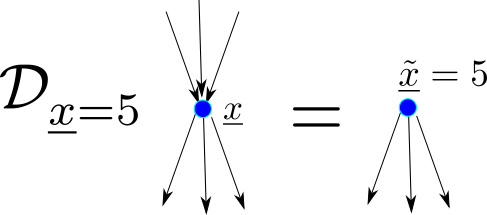
\includegraphics[width=1.75in]
{counterf/rho-op.png}
\caption{Action
of ``do" operator $\cald_{\rvx=5}$
on node $\rvx$.} 
\label{fig-rho-op}
\end{figure}

The do operator $\cald_{\rvx=5}$
is defined graphically in Fig.\ref{fig-rho-op}.
The TPM, printed in blue,
 for node $\tilde{\rvx}$ of Fig.\ref{fig-rho-op},
is as follows.

\beq\color{blue}
P(\tilde{x})=\delta(5, \tilde{x})
\eeq


The do operator $\cald_{\rvx=5}$
amputates
the incoming arrows of node $\rvx$
and sets the TPM
of the new root node $\tilde{\rvx}$
to a delta function $\delta(
\tilde{x}, 5)$
(or some state of $\rvx$
 other than 5).
Sometimes we call the new node
$\cald\rvx$
instead of 
$\tilde{\rvx}$.

The uses of the do operator are discussed
in detail in Chapter \ref{ch-do-calc}.

\section{Imagine operator}

\begin{figure}[h!]
\centering
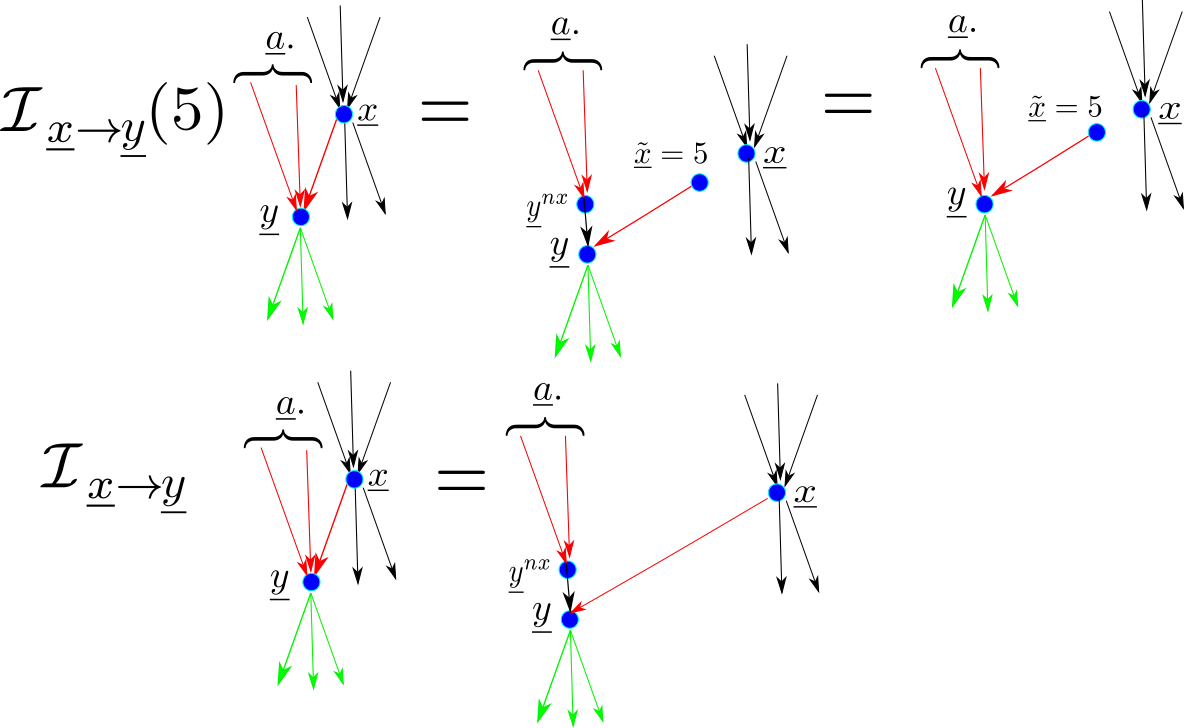
\includegraphics[width=4in]
{counterf/kappa.png}
\caption{Action of ``imagine" operators 
$\cali_{\rvx\rarrow \rvy}(5)$
and $\cali_{\rvx\rarrow \rvy}$
on arrow $\rvx\rarrow \rvy$.
In this figure, $y^{nx}=[y(x)]_{\forall x\in S_\rvx}$,
where $nx=|S_\rvx|$
and $S_\rvx$ is the set of states of node $\rvx$.
} 
\label{fig-kappa}
\end{figure}

The imagine operator  $\cali_{\rvx\rarrow \rvy}(5)$
is defined graphically in Fig.\ref{fig-kappa}.
Note that Fig.\ref{fig-kappa}
actually defines two types 
of imagine operators, the one
with an argument:
$\cali_{\rvx\rarrow \rvy}(5)$,
and the one without an argument: 
$\cali_{\rvx\rarrow \rvy}$.
The TPMs, printed in blue, 
for various nodes in
Fig.\ref{fig-kappa}, are as follows.



\begin{itemize}

\item
For $\cali_{\rvx\rarrow 
\rvy}(\tilde{x})G$

\beq\color{blue}
P(y| \tilde{x}, a.)=
P(y| \rvx=\tilde{x}, a.)
\eeq

\beq\color{blue}
P(\tilde{x})=
\delta(\tilde{x}, 5)
\eeq

\item
For $\cali_{\rvx\rarrow \rvy}G$
\beq\color{blue}
P(y^{nx}| a.)=\prod_{\tilde{x}}
P(\rvy(\tilde{x})=y(\tilde{x})|a.)
\eeq

\beq\color{blue}
P(y|y^{nx}, x)=
\delta(y,y(x))
\eeq
\end{itemize}
The imagine operators 
$\cali_{\rvx\rarrow\rvy}(5)$
and $\cali_{\rvx\rarrow\rvy}$
operate on an arrow
whereas the 
$\cald$ operator
 operates on a node.
$\cali_{\rvx\rarrow\rvy}(5)$
deletes
arrow $\rvx\rarrow\rvy$
and
creates a new root node 
$\tilde{\rvx}$
and a new arrow
$\tilde{\rvx}\rarrow \rvy$.
Sometimes we call
the new node
$\cali_\rvy\rvx$
instead of
 $\tilde{\rvx}$. 
$\cali_{\rvx\rarrow\rvy}$
creates 
a new node $\rvy^{nx}$
and an arrow $\rvy^{nx}\rarrow \rvy$.



\begin{figure}[h!]
$$
\begin{array}{ccccc}
\xymatrix{
&\rvx\ar@[red][ddr]\ar[ddl]
\\
&&&
\\
\rvd\ar@[red][rr]
&
&\rvy\ar@[green][r]
\ar@[green][ur]
&
}
&
\xymatrix{
&&\rvx\ar[ddll]\ar@[red][d]
\\
&&[\rvy(0),\rvy(1)]\ar[d]
&
\\
\rvd\ar@[red][rr]
&
&\rvy\ar@[green][r]
\ar@[green][ur]
&
}
\\
\\
G&G_+=\cali_{\rvd\rarrow\rvy}G
\end{array}
$$
\caption{How 
 imagine operator 
arises in 
Potential Outcomes (PO)
theory.
} 
\label{fig-counterf-G-im-y0-y1}
\end{figure}
Fig.\ref{fig-counterf-G-im-y0-y1}
shows how the
imagine operator arises
in Potential Outcomes (PO) theory.
PO theory is discussed extensively
in Chapter \ref{ch-pot-out}.
As you can see, PO theory
only uses a limited version
of the 3 rungs
of causal inference, because it 
doesn't use the do-operator,
and it only uses one 
of 2 possible types of
imagine operators.
Furthermore,
it assumes a
very limited triangular DAG.


\begin{figure}[h!]
\centering
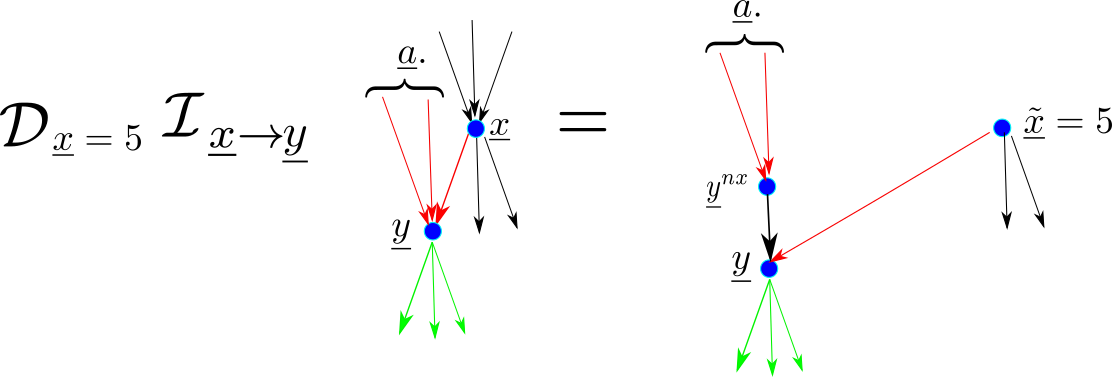
\includegraphics[width=3.5in]
{counterf/rho-kappa.png}
\caption{$\cald_{\rvx=5}\cali_{\rvx\rarrow \rvy}G$
gives a connection
between do and imagine operators.
} 
\label{fig-rho-kappa}
\end{figure}

Fig.\ref{fig-rho-kappa}
gives  a connection
between do and imagine
operators.
We see
from that figure that
for $\cald_{\rvx=\tilde{x}}
\cali_{\rvx\rarrow\rvy}G$, we have\footnote{In the
notation favored by Pearl, Eq.(\ref{eq-connect-do-imag})
 would be
$$P(y|do(X)=\tilde{x}, a.)=P(Y_{\tilde{x}}=y|a.)$$}
\beq
P(y|\cald\rvx=\tilde{x}, a.)=P(\rvy(\tilde{x})=y|a.)
\label{eq-connect-do-imag}
\eeq


One can define
a {\bf do-imagine-calculus}
whose
objective
is to 
express
probabilities such as 
$P(\rvy|\cald\rvr=r,
\cali_\rvb \rvs=s, t)$
in terms of observable 
probabilities
that do not
contain
any do or imagine
operators in them.
As with
Do Calculus,
this reduction
is not 
always possible,
and we say a probability is
{\bf $\cald$-identifiable},
{\bf $\cali$-identifiable}
or
{\bf $\cald\cali$-identifiable}
if it  can be 
expressed without do, imagine
or both operators.

